Prinzipell lässt sich sagen, dass eine Software nur dann für den Endkunden tauglich ist wenn sie reichlich getestet ist. Hierfür gibt es zahlreiche verschiedene Methoden. Vor einiger Zeit wurden die eigentliche Entwicklung der Software und das testen noch als eigenen Prozesse angesehen. Erst mit dem US-amerikanischen Softwareentwickler Kent Beck wurde der Test-First-Ansatz bekannt. Dieser begann einfach den vorherigen Ablauf umzukehren und anstatt mit dem Quellcode zu beginnen schrieb er zuvor einen Test und programmierte dann den dazu benötigten Code. Für einen Laien mag die Testgetriebene Entwicklung am Anfang wohl eher sinnlos erscheinen. Dennoch ist sie sehr effizient, da somit jedes Feature des Quellcodes mit einem Test abgedeckt ist. Außerdem verfasst der Entwickler dann nur so viel Code wie wirklich benötigt wird damit der Test funktioniert.

\begin{figure}
    \centering
    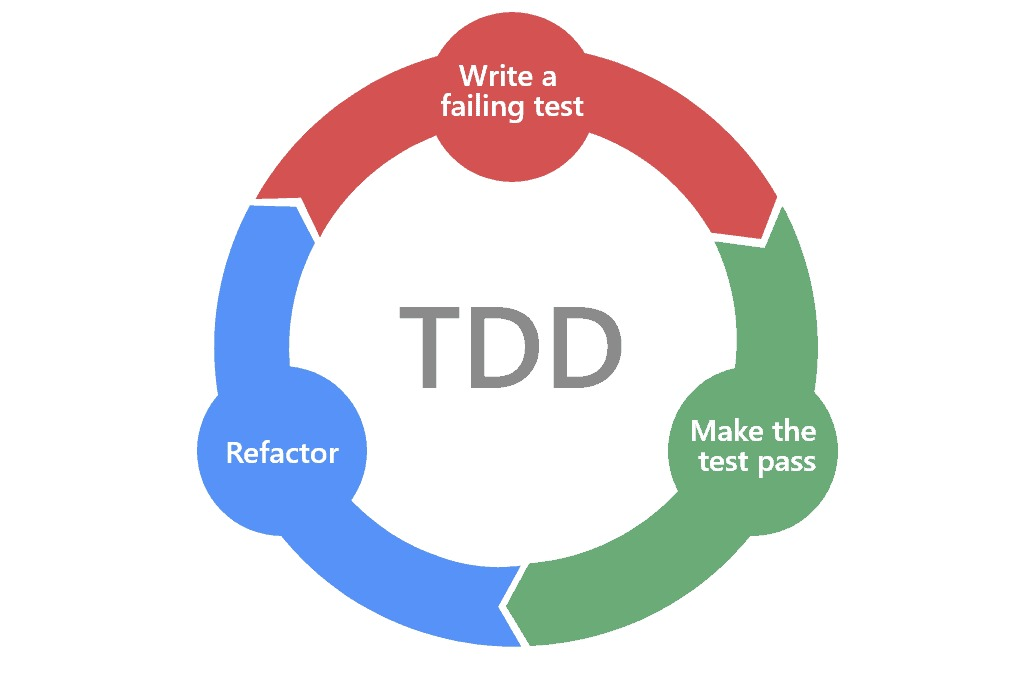
\includegraphics[width=0.5\linewidth]{pics/tdd.jpeg}
    \caption{Wie funktioniert Test Driven Development}
    \label{fig:enter-label}
\end{figure}

\subsection{Wie funktioniert Test Driven Developement genau}

Test Driven Developement (TDD) folgt den Ergebnissen von den schon im vorhinein definierten Testfällen. Mit diesem zyklischen Ansatz wird somit gewährleistet, dass der Code nur dann in das Produktivsystem gelangt, wenn auch alle Anforderungen vom Test erfüllt sind und dieser somit nicht mehr failt. Dies bedeutet, dass der Quellcode so oft überarbeitet werden muss, bis das der Test keine Fehler mehr aufweist. So werden Schrittweise neue Funktionen zum Code hinzufügt. Aus diesem Gründ zählt TDD auch zu den inkrementellen Vorgehensweisen in der Softwareentwicklung.



\cite{Was_ist_TDD}

